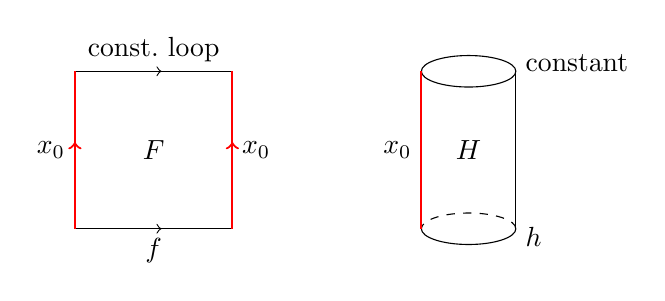
\begin{tikzpicture}
\draw (0,0) -- (2,0) -- (2,2) -- (0,2) -- cycle;
\draw[->] (0,0) -- (1.1,0);
\draw[->] (0,2) -- (1.1,2);
\draw[red, thick, ->] (0,0) -- (0,1.1);
\draw[red, thick] (0,1) -- (0,2);
\draw[red, thick, ->] (2,0) -- (2,1.1);
\draw[red, thick] (2,1) -- (2,2);
\node at (1,1) {$F$};
\node[below] at (1,0) {$f$};
\node[above] at (1,2) {const.\ loop};
\node[left] at (0,1) {$x_0$};
\node[right] at (2,1) {$x_0$};
\node at (3.2,1) {$\rightsquigarrow$};
\draw (5,2) ellipse (0.6 and 0.2);
\draw (4.4,0) arc (180:360:0.6 and 0.2);
\draw[dashed] (5.6,0) arc (0:180:0.6 and 0.2);
\draw[red, thick] (4.4,0) -- (4.4,2);
\draw (5.6,0) -- (5.6,2);
\node at (5,1) {$H$};
\node[left] at (4.4,1) {$x_0$};
\node[right] at (5.6,2.1) {constant};
\node[right] at (5.6,-0.1) {$h$};
\end{tikzpicture}
